\documentclass[twoside]{book}

% Packages required by doxygen
\usepackage{fixltx2e}
\usepackage{calc}
\usepackage{doxygen}
\usepackage[export]{adjustbox} % also loads graphicx
\usepackage{graphicx}
\usepackage[utf8]{inputenc}
\usepackage{makeidx}
\usepackage{multicol}
\usepackage{multirow}
\PassOptionsToPackage{warn}{textcomp}
\usepackage{textcomp}
\usepackage[nointegrals]{wasysym}
\usepackage[table]{xcolor}

% NLS support packages
\usepackage[spanish]{babel}
% Font selection
\usepackage[T1]{fontenc}
\usepackage[scaled=.90]{helvet}
\usepackage{courier}
\usepackage{amssymb}
\usepackage{sectsty}
\renewcommand{\familydefault}{\sfdefault}
\allsectionsfont{%
  \fontseries{bc}\selectfont%
  \color{darkgray}%
}
\renewcommand{\DoxyLabelFont}{%
  \fontseries{bc}\selectfont%
  \color{darkgray}%
}
\newcommand{\+}{\discretionary{\mbox{\scriptsize$\hookleftarrow$}}{}{}}

% Page & text layout
\usepackage{geometry}
\geometry{%
  a4paper,%
  top=2.5cm,%
  bottom=2.5cm,%
  left=2.5cm,%
  right=2.5cm%
}
\tolerance=750
\hfuzz=15pt
\hbadness=750
\setlength{\emergencystretch}{15pt}
\setlength{\parindent}{0cm}
\setlength{\parskip}{3ex plus 2ex minus 2ex}
\makeatletter
\renewcommand{\paragraph}{%
  \@startsection{paragraph}{4}{0ex}{-1.0ex}{1.0ex}{%
    \normalfont\normalsize\bfseries\SS@parafont%
  }%
}
\renewcommand{\subparagraph}{%
  \@startsection{subparagraph}{5}{0ex}{-1.0ex}{1.0ex}{%
    \normalfont\normalsize\bfseries\SS@subparafont%
  }%
}
\makeatother

% Headers & footers
\usepackage{fancyhdr}
\pagestyle{fancyplain}
\fancyhead[LE]{\fancyplain{}{\bfseries\thepage}}
\fancyhead[CE]{\fancyplain{}{}}
\fancyhead[RE]{\fancyplain{}{\bfseries\leftmark}}
\fancyhead[LO]{\fancyplain{}{\bfseries\rightmark}}
\fancyhead[CO]{\fancyplain{}{}}
\fancyhead[RO]{\fancyplain{}{\bfseries\thepage}}
\fancyfoot[LE]{\fancyplain{}{}}
\fancyfoot[CE]{\fancyplain{}{}}
\fancyfoot[RE]{\fancyplain{}{\bfseries\scriptsize Generado por Doxygen }}
\fancyfoot[LO]{\fancyplain{}{\bfseries\scriptsize Generado por Doxygen }}
\fancyfoot[CO]{\fancyplain{}{}}
\fancyfoot[RO]{\fancyplain{}{}}
\renewcommand{\footrulewidth}{0.4pt}
\renewcommand{\chaptermark}[1]{%
  \markboth{#1}{}%
}
\renewcommand{\sectionmark}[1]{%
  \markright{\thesection\ #1}%
}

% Indices & bibliography
\usepackage{natbib}
\usepackage[titles]{tocloft}
\setcounter{tocdepth}{3}
\setcounter{secnumdepth}{5}
\makeindex

% Hyperlinks (required, but should be loaded last)
\usepackage{ifpdf}
\ifpdf
  \usepackage[pdftex,pagebackref=true]{hyperref}
\else
  \usepackage[ps2pdf,pagebackref=true]{hyperref}
\fi
\hypersetup{%
  colorlinks=true,%
  linkcolor=blue,%
  citecolor=blue,%
  unicode%
}

% Custom commands
\newcommand{\clearemptydoublepage}{%
  \newpage{\pagestyle{empty}\cleardoublepage}%
}

\usepackage{caption}
\captionsetup{labelsep=space,justification=centering,font={bf},singlelinecheck=off,skip=4pt,position=top}

%===== C O N T E N T S =====

\begin{document}

% Titlepage & ToC
\hypersetup{pageanchor=false,
             bookmarksnumbered=true,
             pdfencoding=unicode
            }
\pagenumbering{roman}
\begin{titlepage}
\vspace*{7cm}
\begin{center}%
{\Large Laboratorio de P\+R\+O2. Tree\+K\+EA. \\[1ex]\large version 3 03-\/may-\/2018 }\\
\vspace*{1cm}
{\large Generado por Doxygen 1.8.11}\\
\end{center}
\end{titlepage}
\clearemptydoublepage
\tableofcontents
\clearemptydoublepage
\pagenumbering{arabic}
\hypersetup{pageanchor=true}

%--- Begin generated contents ---
\chapter{Página principal}
\label{index}\hypertarget{index}{}El programa principal se encuentra en el módulo \hyperlink{pro2_8cc}{pro2.\+cc}.

Atendiendo a los tipos de datos sugeridos en el enunciado, necesitaremos dos módulos\+: un módulo para representar el almacén y otro para representar una sala.

La simulacion se plantea como un almacén contenedor de un conjunto de salas y un registro de productos global (incluido en el almacén). 
\chapter{Índice de clases}
\section{Lista de clases}
Lista de las clases, estructuras, uniones e interfaces con una breve descripción\+:\begin{DoxyCompactList}
\item\contentsline{section}{\hyperlink{class_cubeta}{Cubeta} \\*Representa una cubeta de ropa }{\pageref{class_cubeta}}{}
\item\contentsline{section}{\hyperlink{class_lavadora}{Lavadora} \\*Representa una lavadora }{\pageref{class_lavadora}}{}
\item\contentsline{section}{\hyperlink{class_prenda}{Prenda} \\*Representa una prenda de ropa con atributos peso y color }{\pageref{class_prenda}}{}
\end{DoxyCompactList}

\chapter{Indice de archivos}
\section{Lista de archivos}
Lista de todos los archivos con descripciones breves\+:\begin{DoxyCompactList}
\item\contentsline{section}{\hyperlink{_cubeta_8hh}{Cubeta.\+hh} \\*Especificación de la clase \hyperlink{class_cubeta}{Cubeta} }{\pageref{_cubeta_8hh}}{}
\item\contentsline{section}{\hyperlink{_lavadora_8hh}{Lavadora.\+hh} \\*Especificación de la clase \hyperlink{class_lavadora}{Lavadora} }{\pageref{_lavadora_8hh}}{}
\item\contentsline{section}{\hyperlink{_prenda_8hh}{Prenda.\+hh} \\*Especificación de la clase \hyperlink{class_prenda}{Prenda} }{\pageref{_prenda_8hh}}{}
\item\contentsline{section}{\hyperlink{pro2__s8_8cc}{pro2\+\_\+s8.\+cc} \\*Programa principal para el ejercicio {\itshape Gestión de una lavadora} }{\pageref{pro2__s8_8cc}}{}
\item\contentsline{section}{\hyperlink{readbool_8hh}{readbool.\+hh} \\*Operacion para leer booleanos del canal estandar }{\pageref{readbool_8hh}}{}
\end{DoxyCompactList}

\chapter{Documentación de las clases}
\hypertarget{class_almacen}{}\section{Referencia de la Clase Almacen}
\label{class_almacen}\index{Almacen@{Almacen}}


Representa el almacén virtual que contiene en su interior el conjunto completo de salas. A su vez el almacén cuenta con un registro de todos los productos que contiene con sus respectivas cantidades.  


\subsection*{Métodos públicos}
\begin{DoxyCompactItemize}
\item 
\hyperlink{class_almacen_ab6569f621c050df752fcdf5e1614631e}{Almacen} (int N)
\begin{DoxyCompactList}\small\item\em Creadora de un almacén estructurado y completado con N salas asociadas cada una a un identificador. \end{DoxyCompactList}\item 
void \hyperlink{class_almacen_a5ceb8f70af951fdd3c961e693fa2f53d}{poner\+\_\+prod} (const string \&prod)
\begin{DoxyCompactList}\small\item\em Modificadora que añade un producto a la lista de productos. \end{DoxyCompactList}\item 
void \hyperlink{class_almacen_a1899609156ebe6d1bca071dd4fea5eb2}{quitar\+\_\+prod} (const string \&prod)
\begin{DoxyCompactList}\small\item\em Modificadora que elimina un producto a la lista de productos. \end{DoxyCompactList}\item 
int \hyperlink{class_almacen_a0718beb9b0ed5272d030ac2c0b72364d}{poner\+\_\+items} (int s, const string \&prod, int cant)
\begin{DoxyCompactList}\small\item\em Modificadora que añade una cantidad concreta de un producto a una sala concreta. \end{DoxyCompactList}\item 
int \hyperlink{class_almacen_a16de14cab27a1789eeecc23abfeacc5a}{quitar\+\_\+items} (int s, const string \&prod, int cant)
\begin{DoxyCompactList}\small\item\em Modificadora que quita una cantidad concreta de un producto a una sala concreta. \end{DoxyCompactList}\item 
int \hyperlink{class_almacen_acfd635dc057df10be22e9920ecca607b}{distribuir} (const string \&prod, int cant)
\begin{DoxyCompactList}\small\item\em Modificadora que distribuye una cantidad de productos por el almacén y retorna la cantidad sobrante. \end{DoxyCompactList}\item 
void \hyperlink{class_almacen_a2e6c76cf94ab9a0a9436df2fadd71dd2}{compactar} (int s)
\begin{DoxyCompactList}\small\item\em Modificadora de una sala que compacta todos los items de la estantería que contiene. \end{DoxyCompactList}\item 
void \hyperlink{class_almacen_acb6e13d2501688e17607b4a74fb18cf8}{reorganizar} (int s)
\begin{DoxyCompactList}\small\item\em Modificadora de una sala que ordena todos los elementos de la estantería que contiene por orden alfabético. \end{DoxyCompactList}\item 
bool \hyperlink{class_almacen_a873095b67a174bc27fd473043fef2a25}{redimensionar} (int s, int fil, int col)
\begin{DoxyCompactList}\small\item\em Modificadora de una sala que, si puede, modifica las dimensiones de la estantería que contiene. \end{DoxyCompactList}\item 
void \hyperlink{class_almacen_a25ae2690b3295f66fa5798c01b7ab182}{lectura\+\_\+dimensiones\+\_\+salas} ()
\begin{DoxyCompactList}\small\item\em Modificadora lee las dimensiones de las salas contenidas en el parámetro implícito por orden de identificador. \end{DoxyCompactList}\item 
void \hyperlink{class_almacen_affa9fb3647b6cdb13184371dd9e32454}{inventario} ()
\begin{DoxyCompactList}\small\item\em Consultora que imprime por pantalla la lista de productos y cantidades por orden alfabético. \end{DoxyCompactList}\item 
void \hyperlink{class_almacen_adabb9eae94dd8fb804f2eea351c175fa}{escribir} (int s)
\begin{DoxyCompactList}\small\item\em Consultora que imprime por pantalla la estantería de la sala solicitada. \end{DoxyCompactList}\item 
string \hyperlink{class_almacen_acc3d87560515901a960413e8c3efd0ae}{consultar\+\_\+pos} (int s, int i, int j)
\begin{DoxyCompactList}\small\item\em Consultora que retorna el item que se encuentra en una posicion concreta de la estantería, contenida en una sala. \end{DoxyCompactList}\item 
int \hyperlink{class_almacen_a8a6da3c276db98363302e50f9fe4b22a}{consultar\+\_\+prod} (const string \&prod)
\begin{DoxyCompactList}\small\item\em Consultora retorna la cantidad que hay de un producto. \end{DoxyCompactList}\end{DoxyCompactItemize}


\subsection{Descripción detallada}
Representa el almacén virtual que contiene en su interior el conjunto completo de salas. A su vez el almacén cuenta con un registro de todos los productos que contiene con sus respectivas cantidades. 

Ofrece operaciones tanto como para modificar como para consultar el contenido de las salas y la lista o registro de productos de nuestro sistema. 

Definición en la línea 32 del archivo Almacen.\+hh.



\subsection{Documentación del constructor y destructor}
\index{Almacen@{Almacen}!Almacen@{Almacen}}
\index{Almacen@{Almacen}!Almacen@{Almacen}}
\subsubsection[{\texorpdfstring{Almacen(int N)}{Almacen(int N)}}]{\setlength{\rightskip}{0pt plus 5cm}Almacen\+::\+Almacen (
\begin{DoxyParamCaption}
\item[{int}]{N}
\end{DoxyParamCaption}
)}\hypertarget{class_almacen_ab6569f621c050df752fcdf5e1614631e}{}\label{class_almacen_ab6569f621c050df752fcdf5e1614631e}


Creadora de un almacén estructurado y completado con N salas asociadas cada una a un identificador. 

\begin{DoxyPrecond}{Precondición}
N es un entero positivo. 
\end{DoxyPrecond}
\begin{DoxyPostcond}{Postcondición}
El parámetro implícito esta estructurado y completado con N salas asociadas cada una a un identificador. 
\end{DoxyPostcond}
\begin{DoxyParagraph}{Coste}
Lineal 
\end{DoxyParagraph}


\subsection{Documentación de las funciones miembro}
\index{Almacen@{Almacen}!poner\+\_\+prod@{poner\+\_\+prod}}
\index{poner\+\_\+prod@{poner\+\_\+prod}!Almacen@{Almacen}}
\subsubsection[{\texorpdfstring{poner\+\_\+prod(const string \&prod)}{poner_prod(const string &prod)}}]{\setlength{\rightskip}{0pt plus 5cm}void Almacen\+::poner\+\_\+prod (
\begin{DoxyParamCaption}
\item[{const string \&}]{prod}
\end{DoxyParamCaption}
)}\hypertarget{class_almacen_a5ceb8f70af951fdd3c961e693fa2f53d}{}\label{class_almacen_a5ceb8f70af951fdd3c961e693fa2f53d}


Modificadora que añade un producto a la lista de productos. 

\begin{DoxyPrecond}{Precondición}
Cierto. 
\end{DoxyPrecond}
\begin{DoxyPostcond}{Postcondición}
La lista de productos del parámetro implícito se mantiene igual y contiene el producto {\itshape prod}. Si previamente lo contenia se produce un error. 
\end{DoxyPostcond}
\begin{DoxyParagraph}{Coste}
Constante. 
\end{DoxyParagraph}
\index{Almacen@{Almacen}!quitar\+\_\+prod@{quitar\+\_\+prod}}
\index{quitar\+\_\+prod@{quitar\+\_\+prod}!Almacen@{Almacen}}
\subsubsection[{\texorpdfstring{quitar\+\_\+prod(const string \&prod)}{quitar_prod(const string &prod)}}]{\setlength{\rightskip}{0pt plus 5cm}void Almacen\+::quitar\+\_\+prod (
\begin{DoxyParamCaption}
\item[{const string \&}]{prod}
\end{DoxyParamCaption}
)}\hypertarget{class_almacen_a1899609156ebe6d1bca071dd4fea5eb2}{}\label{class_almacen_a1899609156ebe6d1bca071dd4fea5eb2}


Modificadora que elimina un producto a la lista de productos. 

\begin{DoxyPrecond}{Precondición}
Cierto. 
\end{DoxyPrecond}
\begin{DoxyPostcond}{Postcondición}
La lista de productos del parámetro implícito se mantiene igual pero sin el producto {\itshape prod}. Si previamente no estaba contenido se produce un error. 
\end{DoxyPostcond}
\begin{DoxyParagraph}{Coste}
Constante. 
\end{DoxyParagraph}
\index{Almacen@{Almacen}!poner\+\_\+items@{poner\+\_\+items}}
\index{poner\+\_\+items@{poner\+\_\+items}!Almacen@{Almacen}}
\subsubsection[{\texorpdfstring{poner\+\_\+items(int s, const string \&prod, int cant)}{poner_items(int s, const string &prod, int cant)}}]{\setlength{\rightskip}{0pt plus 5cm}int Almacen\+::poner\+\_\+items (
\begin{DoxyParamCaption}
\item[{int}]{s, }
\item[{const string \&}]{prod, }
\item[{int}]{cant}
\end{DoxyParamCaption}
)}\hypertarget{class_almacen_a0718beb9b0ed5272d030ac2c0b72364d}{}\label{class_almacen_a0718beb9b0ed5272d030ac2c0b72364d}


Modificadora que añade una cantidad concreta de un producto a una sala concreta. 

\begin{DoxyPrecond}{Precondición}
El identificador de sala {\itshape s} pertenece a una sala que existe y la cantidad {\itshape cant} es positiva. 
\end{DoxyPrecond}
\begin{DoxyPostcond}{Postcondición}
Si el producto no existe se produce un error. Si existe, la estantería de la sala contenida en el parámetro implícito ha sido llenada con una cantidad {\itshape cant} de productos {\itshape prod} o bien hasta que se ha llenado la estaneria o bien hasta que se haya agotado la susodicha cantidad. El rellenado se habra realizado llenando primero los huecos a partir del hueco que fuera antes. Se retorna la cantidad de items que no cabian en la estantería o un -\/1 en caso de producirse un error. 
\end{DoxyPostcond}
\begin{DoxyParagraph}{Coste}
Lineal. 
\end{DoxyParagraph}
\index{Almacen@{Almacen}!quitar\+\_\+items@{quitar\+\_\+items}}
\index{quitar\+\_\+items@{quitar\+\_\+items}!Almacen@{Almacen}}
\subsubsection[{\texorpdfstring{quitar\+\_\+items(int s, const string \&prod, int cant)}{quitar_items(int s, const string &prod, int cant)}}]{\setlength{\rightskip}{0pt plus 5cm}int Almacen\+::quitar\+\_\+items (
\begin{DoxyParamCaption}
\item[{int}]{s, }
\item[{const string \&}]{prod, }
\item[{int}]{cant}
\end{DoxyParamCaption}
)}\hypertarget{class_almacen_a16de14cab27a1789eeecc23abfeacc5a}{}\label{class_almacen_a16de14cab27a1789eeecc23abfeacc5a}


Modificadora que quita una cantidad concreta de un producto a una sala concreta. 

\begin{DoxyPrecond}{Precondición}
El identificador de sala {\itshape s} pertenece a una sala que existe y la cantidad {\itshape cant} es positiva. 
\end{DoxyPrecond}
\begin{DoxyPostcond}{Postcondición}
Si el producto no existe se produce un error. Se quita de la estaneria de la sala contenida en el parámetro implícito una cantidad {\itshape cant} de productos {\itshape prod} empezando por el producto que vaya antes. Se retorna la cantidad de items que no se han podido quitar o un -\/1 en caso de producirse un error. 
\end{DoxyPostcond}
\begin{DoxyParagraph}{Coste}
Lineal. 
\end{DoxyParagraph}
\index{Almacen@{Almacen}!distribuir@{distribuir}}
\index{distribuir@{distribuir}!Almacen@{Almacen}}
\subsubsection[{\texorpdfstring{distribuir(const string \&prod, int cant)}{distribuir(const string &prod, int cant)}}]{\setlength{\rightskip}{0pt plus 5cm}int Almacen\+::distribuir (
\begin{DoxyParamCaption}
\item[{const string \&}]{prod, }
\item[{int}]{cant}
\end{DoxyParamCaption}
)}\hypertarget{class_almacen_acfd635dc057df10be22e9920ecca607b}{}\label{class_almacen_acfd635dc057df10be22e9920ecca607b}


Modificadora que distribuye una cantidad de productos por el almacén y retorna la cantidad sobrante. 

\begin{DoxyPrecond}{Precondición}
La cantidad {\itshape cant} de productos {\itshape prod} es positiva.
\end{DoxyPrecond}
\begin{DoxyPostcond}{Postcondición}
Se han distribuido una cantidad {\itshape cant} de productos {\itshape prod} por las diferentes salas segun un ($\ast$)criterio y se retorna la cantidad de productos no añadidos.
\end{DoxyPostcond}
($\ast$)Criterio (jerárquico)\+:

(1) Hay que añadir tantos productos como cantidad del mismo definida.

(2) Si el parámetro implícito esta lleno, se finaliza el proceso.

(3) Se empieza por la primera sala, si esta se llena (o lo estaba previamente) se divide la cantidad C que queda por repartir en 2 partes iguales A y B (si la cantidad C es impar, se cumplirá A+1 = B). La cantidad A va la sala de la izquierda, y la cantidad B a la sala de la derecha. Sucesivamente, aplicamos a cada sala el mismo proceso y criterio.

\begin{DoxyParagraph}{Coste}
Lineal. 
\end{DoxyParagraph}
\index{Almacen@{Almacen}!compactar@{compactar}}
\index{compactar@{compactar}!Almacen@{Almacen}}
\subsubsection[{\texorpdfstring{compactar(int s)}{compactar(int s)}}]{\setlength{\rightskip}{0pt plus 5cm}void Almacen\+::compactar (
\begin{DoxyParamCaption}
\item[{int}]{s}
\end{DoxyParamCaption}
)}\hypertarget{class_almacen_a2e6c76cf94ab9a0a9436df2fadd71dd2}{}\label{class_almacen_a2e6c76cf94ab9a0a9436df2fadd71dd2}


Modificadora de una sala que compacta todos los items de la estantería que contiene. 

\begin{DoxyPrecond}{Precondición}
El identificador de sala {\itshape s} pertenece a una sala que existe. 
\end{DoxyPrecond}
\begin{DoxyPostcond}{Postcondición}
Todos los items de la estantería contenida en la sala del parámetro implícito quedan agrupados (sin espacios vacíos entre ellos) lo mas abajo y a la izquierda posible de la misma y manteniendo el orden previo. 
\end{DoxyPostcond}
\begin{DoxyParagraph}{Coste}
Lineal. 
\end{DoxyParagraph}
\index{Almacen@{Almacen}!reorganizar@{reorganizar}}
\index{reorganizar@{reorganizar}!Almacen@{Almacen}}
\subsubsection[{\texorpdfstring{reorganizar(int s)}{reorganizar(int s)}}]{\setlength{\rightskip}{0pt plus 5cm}void Almacen\+::reorganizar (
\begin{DoxyParamCaption}
\item[{int}]{s}
\end{DoxyParamCaption}
)}\hypertarget{class_almacen_acb6e13d2501688e17607b4a74fb18cf8}{}\label{class_almacen_acb6e13d2501688e17607b4a74fb18cf8}


Modificadora de una sala que ordena todos los elementos de la estantería que contiene por orden alfabético. 

\begin{DoxyPrecond}{Precondición}
El identificador de sala {\itshape s} pertenece a una sala que existe. 
\end{DoxyPrecond}
\begin{DoxyPostcond}{Postcondición}
La sala {\itshape s} del parámetro implícito tiene los items de la estantería compactados y ordenados alfabeticamente segun el identificador de producto. 
\end{DoxyPostcond}
\begin{DoxyParagraph}{Coste}
Logarítmico. 
\end{DoxyParagraph}
\index{Almacen@{Almacen}!redimensionar@{redimensionar}}
\index{redimensionar@{redimensionar}!Almacen@{Almacen}}
\subsubsection[{\texorpdfstring{redimensionar(int s, int fil, int col)}{redimensionar(int s, int fil, int col)}}]{\setlength{\rightskip}{0pt plus 5cm}bool Almacen\+::redimensionar (
\begin{DoxyParamCaption}
\item[{int}]{s, }
\item[{int}]{fil, }
\item[{int}]{col}
\end{DoxyParamCaption}
)}\hypertarget{class_almacen_a873095b67a174bc27fd473043fef2a25}{}\label{class_almacen_a873095b67a174bc27fd473043fef2a25}


Modificadora de una sala que, si puede, modifica las dimensiones de la estantería que contiene. 

\begin{DoxyPrecond}{Precondición}
El identificador de sala {\itshape s} pertenece a una sala que existe y los enteros {\itshape fil} y {\itshape col} son positivos o iguales a 0. 
\end{DoxyPrecond}
\begin{DoxyPostcond}{Postcondición}
Si la cantidad de items cabe en las nuevas dimensiones, la estantería contenida en la sala del parámetro implícito queda redimensionada a {\itshape fil x col} y tiene los items compactados. Por contra, si la cantidad de items no cabe en las nuevas dimensiones, se produce un error y el parámetro implícito permanece igual. 
\end{DoxyPostcond}
\begin{DoxyParagraph}{Coste}
Lineal. 
\end{DoxyParagraph}
\index{Almacen@{Almacen}!lectura\+\_\+dimensiones\+\_\+salas@{lectura\+\_\+dimensiones\+\_\+salas}}
\index{lectura\+\_\+dimensiones\+\_\+salas@{lectura\+\_\+dimensiones\+\_\+salas}!Almacen@{Almacen}}
\subsubsection[{\texorpdfstring{lectura\+\_\+dimensiones\+\_\+salas()}{lectura_dimensiones_salas()}}]{\setlength{\rightskip}{0pt plus 5cm}void Almacen\+::lectura\+\_\+dimensiones\+\_\+salas (
\begin{DoxyParamCaption}
{}
\end{DoxyParamCaption}
)}\hypertarget{class_almacen_a25ae2690b3295f66fa5798c01b7ab182}{}\label{class_almacen_a25ae2690b3295f66fa5798c01b7ab182}


Modificadora lee las dimensiones de las salas contenidas en el parámetro implícito por orden de identificador. 

\begin{DoxyPrecond}{Precondición}
Cierto. 
\end{DoxyPrecond}
\begin{DoxyPostcond}{Postcondición}
Todas las salas del parámetro implícito contienen una estantería dimensionada vacia. 
\end{DoxyPostcond}
\begin{DoxyParagraph}{Coste}
Lineal. 
\end{DoxyParagraph}
\index{Almacen@{Almacen}!inventario@{inventario}}
\index{inventario@{inventario}!Almacen@{Almacen}}
\subsubsection[{\texorpdfstring{inventario()}{inventario()}}]{\setlength{\rightskip}{0pt plus 5cm}void Almacen\+::inventario (
\begin{DoxyParamCaption}
{}
\end{DoxyParamCaption}
)}\hypertarget{class_almacen_affa9fb3647b6cdb13184371dd9e32454}{}\label{class_almacen_affa9fb3647b6cdb13184371dd9e32454}


Consultora que imprime por pantalla la lista de productos y cantidades por orden alfabético. 

\begin{DoxyPrecond}{Precondición}
Cierto. 
\end{DoxyPrecond}
\begin{DoxyPostcond}{Postcondición}
Se escriben los identificadores de los todos productos y sus respectivas cantidades por orden alfabético. 
\end{DoxyPostcond}
\begin{DoxyParagraph}{Coste}
Lineal. 
\end{DoxyParagraph}
\index{Almacen@{Almacen}!escribir@{escribir}}
\index{escribir@{escribir}!Almacen@{Almacen}}
\subsubsection[{\texorpdfstring{escribir(int s)}{escribir(int s)}}]{\setlength{\rightskip}{0pt plus 5cm}void Almacen\+::escribir (
\begin{DoxyParamCaption}
\item[{int}]{s}
\end{DoxyParamCaption}
)}\hypertarget{class_almacen_adabb9eae94dd8fb804f2eea351c175fa}{}\label{class_almacen_adabb9eae94dd8fb804f2eea351c175fa}


Consultora que imprime por pantalla la estantería de la sala solicitada. 

\begin{DoxyPrecond}{Precondición}
El identificador de sala {\itshape s} pertenece a una sala que existe. 
\end{DoxyPrecond}
\begin{DoxyPostcond}{Postcondición}
Se imprime por pantalla, tal y como estan posicionados en la estantería, el conenido de cada una de las celdas de la estantería de la sala {\itshape s}. Si hay un item, se imprime su identificar. Si hay un hueco vacío, se imprime N\+U\+LL. 
\end{DoxyPostcond}
\begin{DoxyParagraph}{Coste}
Lineal. 
\end{DoxyParagraph}
\index{Almacen@{Almacen}!consultar\+\_\+pos@{consultar\+\_\+pos}}
\index{consultar\+\_\+pos@{consultar\+\_\+pos}!Almacen@{Almacen}}
\subsubsection[{\texorpdfstring{consultar\+\_\+pos(int s, int i, int j)}{consultar_pos(int s, int i, int j)}}]{\setlength{\rightskip}{0pt plus 5cm}string Almacen\+::consultar\+\_\+pos (
\begin{DoxyParamCaption}
\item[{int}]{s, }
\item[{int}]{i, }
\item[{int}]{j}
\end{DoxyParamCaption}
)}\hypertarget{class_almacen_acc3d87560515901a960413e8c3efd0ae}{}\label{class_almacen_acc3d87560515901a960413e8c3efd0ae}


Consultora que retorna el item que se encuentra en una posicion concreta de la estantería, contenida en una sala. 

\begin{DoxyPrecond}{Precondición}
El identificador de sala {\itshape s} pertenece a una sala que existe. Los enteros {\itshape i} y {\itshape j} se encuentran dentro del rango (0, F\+I\+L\+AS) y (0, C\+O\+L\+U\+M\+N\+AS) respectivamente, donde F\+I\+L\+AS es el numero total de filas -\/ 1 y C\+O\+L\+U\+M\+N\+AS es el numero total de columnas -\/ 1 de la estaneria. 
\end{DoxyPrecond}
\begin{DoxyPostcond}{Postcondición}
Se retorna el identificador del item que se encuentra en la posicion i-\/j de la sala s. Si dicha posicion esta vacia se retorna \char`\"{}\+N\+U\+L\+L\char`\"{}. 
\end{DoxyPostcond}
\begin{DoxyParagraph}{Coste}
Lineal. 
\end{DoxyParagraph}
\index{Almacen@{Almacen}!consultar\+\_\+prod@{consultar\+\_\+prod}}
\index{consultar\+\_\+prod@{consultar\+\_\+prod}!Almacen@{Almacen}}
\subsubsection[{\texorpdfstring{consultar\+\_\+prod(const string \&prod)}{consultar_prod(const string &prod)}}]{\setlength{\rightskip}{0pt plus 5cm}int Almacen\+::consultar\+\_\+prod (
\begin{DoxyParamCaption}
\item[{const string \&}]{prod}
\end{DoxyParamCaption}
)}\hypertarget{class_almacen_a8a6da3c276db98363302e50f9fe4b22a}{}\label{class_almacen_a8a6da3c276db98363302e50f9fe4b22a}


Consultora retorna la cantidad que hay de un producto. 

\begin{DoxyPrecond}{Precondición}
Cierto. 
\end{DoxyPrecond}
\begin{DoxyPostcond}{Postcondición}
Se retorna la cantidad de items del producto {\itshape prod}. En caso de que el prodcuto no este en la lista de productos, se retorna un -\/1. 
\end{DoxyPostcond}
\begin{DoxyParagraph}{Coste}
Constante. 
\end{DoxyParagraph}


La documentación para esta clase fue generada a partir del siguiente fichero\+:\begin{DoxyCompactItemize}
\item 
\hyperlink{_almacen_8hh}{Almacen.\+hh}\end{DoxyCompactItemize}

\hypertarget{class_sala}{}\section{Referencia de la Clase Sala}
\label{class_sala}\index{Sala@{Sala}}


Representa una sala virtual asociada a un identificador y que contiene una estantería junto a datos relacionadas con la misma\+: dimensiones, espacio ocupado y espacio máximo.  


\subsection*{Métodos públicos}
\begin{DoxyCompactItemize}
\item 
\hyperlink{class_sala_ab6f672b31658edd49b5d409bf9fbe659}{Sala} (int id)
\begin{DoxyCompactList}\small\item\em Creadora de \hyperlink{class_sala}{Sala} asociada a un identificador. \end{DoxyCompactList}\item 
void \hyperlink{class_sala_a748f6e7dd49a9c5f67623640f774e0ff}{poner\+\_\+items} (const string \&prod, int cant)
\begin{DoxyCompactList}\small\item\em Modificadora que añade una cantidad concreta de items a una estantería. \end{DoxyCompactList}\item 
void \hyperlink{class_sala_a4e449719446b07b4626c8502a87a5af2}{quitar\+\_\+items} (const string \&prod, int cant)
\begin{DoxyCompactList}\small\item\em Modificadora que quita una cantidad concreta de items a una estantería. \end{DoxyCompactList}\item 
void \hyperlink{class_sala_aac11486a22560bdcdb7771e9692cfa75}{compactar} ()
\begin{DoxyCompactList}\small\item\em Modificadora que compacta todos los elementos de la estantería del parámetro implicito. \end{DoxyCompactList}\item 
void \hyperlink{class_sala_aaac8d848595b493ea08516f2101b829e}{reorganizar} ()
\begin{DoxyCompactList}\small\item\em Modificadora que ordena alfabeticamente (segun su identificador) todos los elementos de la estantería del parámetro implicito. \end{DoxyCompactList}\item 
bool \hyperlink{class_sala_abed3d192d416f7f14be6e8597f5e6059}{redimensionar} (int fil, int col)
\begin{DoxyCompactList}\small\item\em Modificadora que, si los items que contiene la estaneria caben en las nuevas dimensiones, modifica las dimensiones de la misma y compacta los items. \end{DoxyCompactList}\item 
void \hyperlink{class_sala_a1b8b14baf2acaf5a118fc0e426fc107d}{asignacion\+\_\+dimensiones\+\_\+estanteria} (int filas, int columnas)
\begin{DoxyCompactList}\small\item\em Modificadora que otorga las características espaciales a una estaneria adimensionada. \end{DoxyCompactList}\item 
void \hyperlink{class_sala_afd8421dde833322ed676c232e88cb77c}{escribir} ()
\begin{DoxyCompactList}\small\item\em Consultora encargada de imprimir por pantalla la estaneria del parámetro implicito. \end{DoxyCompactList}\item 
string \hyperlink{class_sala_acb7088c40e1720d1604fc37a4d10443b}{consultar\+\_\+pos} (int i, int j)
\begin{DoxyCompactList}\small\item\em Consultora que retorna el identificador del item que se encuentra en una posicion concreta. \end{DoxyCompactList}\end{DoxyCompactItemize}


\subsection{Descripción detallada}
Representa una sala virtual asociada a un identificador y que contiene una estantería junto a datos relacionadas con la misma\+: dimensiones, espacio ocupado y espacio máximo. 

Ofrece operaciones para modificar el contenido de las estanterías así como las variables asociadas a la misma y citadas previamente. 

Definición en la línea 31 del archivo Sala.\+hh.



\subsection{Documentación del constructor y destructor}
\index{Sala@{Sala}!Sala@{Sala}}
\index{Sala@{Sala}!Sala@{Sala}}
\subsubsection[{\texorpdfstring{Sala(int id)}{Sala(int id)}}]{\setlength{\rightskip}{0pt plus 5cm}Sala\+::\+Sala (
\begin{DoxyParamCaption}
\item[{int}]{id}
\end{DoxyParamCaption}
)}\hypertarget{class_sala_ab6f672b31658edd49b5d409bf9fbe659}{}\label{class_sala_ab6f672b31658edd49b5d409bf9fbe659}


Creadora de \hyperlink{class_sala}{Sala} asociada a un identificador. 

\begin{DoxyPrecond}{Precondición}
El identificador es un entero positivo y diferente de cero. 
\end{DoxyPrecond}
\begin{DoxyPostcond}{Postcondición}
El resultado es una sala asociada al identificador {\itshape id} con una estantería vacía y de tamaño cero. 
\end{DoxyPostcond}
\begin{DoxyParagraph}{Coste}
Constante. 
\end{DoxyParagraph}


\subsection{Documentación de las funciones miembro}
\index{Sala@{Sala}!poner\+\_\+items@{poner\+\_\+items}}
\index{poner\+\_\+items@{poner\+\_\+items}!Sala@{Sala}}
\subsubsection[{\texorpdfstring{poner\+\_\+items(const string \&prod, int cant)}{poner_items(const string &prod, int cant)}}]{\setlength{\rightskip}{0pt plus 5cm}void Sala\+::poner\+\_\+items (
\begin{DoxyParamCaption}
\item[{const string \&}]{prod, }
\item[{int}]{cant}
\end{DoxyParamCaption}
)}\hypertarget{class_sala_a748f6e7dd49a9c5f67623640f774e0ff}{}\label{class_sala_a748f6e7dd49a9c5f67623640f774e0ff}


Modificadora que añade una cantidad concreta de items a una estantería. 

\begin{DoxyPrecond}{Precondición}
La cantidad {\itshape cant} es positiva. 
\end{DoxyPrecond}
\begin{DoxyPostcond}{Postcondición}
la estantería contenida en el parámetro implícito ha sido llenada con una cantidad {\itshape cant} de productos {\itshape prod} o bien hasta que se ha llenado la estaneria o bien hasta que se haya agotado la susodicha cantidad. El rellenado se habra realizado llenando primero los huecos a partir del hueco que fuera antes. 
\end{DoxyPostcond}
\begin{DoxyParagraph}{Coste}
Lineal. 
\end{DoxyParagraph}
\index{Sala@{Sala}!quitar\+\_\+items@{quitar\+\_\+items}}
\index{quitar\+\_\+items@{quitar\+\_\+items}!Sala@{Sala}}
\subsubsection[{\texorpdfstring{quitar\+\_\+items(const string \&prod, int cant)}{quitar_items(const string &prod, int cant)}}]{\setlength{\rightskip}{0pt plus 5cm}void Sala\+::quitar\+\_\+items (
\begin{DoxyParamCaption}
\item[{const string \&}]{prod, }
\item[{int}]{cant}
\end{DoxyParamCaption}
)}\hypertarget{class_sala_a4e449719446b07b4626c8502a87a5af2}{}\label{class_sala_a4e449719446b07b4626c8502a87a5af2}


Modificadora que quita una cantidad concreta de items a una estantería. 

\begin{DoxyPrecond}{Precondición}
La cantidad {\itshape cant} es positiva. 
\end{DoxyPrecond}
\begin{DoxyPostcond}{Postcondición}
A la estantería contenida en el parámetro implícito le ha sido retirada una cantidad {\itshape cant} de productos {\itshape prod} o bien hasta que se ha llenado la estaneria o bien hasta que se haya agotado la susodicha cantidad. La acción se habra realizado quitando primero los items que vayan antes. 
\end{DoxyPostcond}
\begin{DoxyParagraph}{Coste}
Lineal. 
\end{DoxyParagraph}
\index{Sala@{Sala}!compactar@{compactar}}
\index{compactar@{compactar}!Sala@{Sala}}
\subsubsection[{\texorpdfstring{compactar()}{compactar()}}]{\setlength{\rightskip}{0pt plus 5cm}void Sala\+::compactar (
\begin{DoxyParamCaption}
{}
\end{DoxyParamCaption}
)}\hypertarget{class_sala_aac11486a22560bdcdb7771e9692cfa75}{}\label{class_sala_aac11486a22560bdcdb7771e9692cfa75}


Modificadora que compacta todos los elementos de la estantería del parámetro implicito. 

\begin{DoxyPrecond}{Precondición}
Cierto. 
\end{DoxyPrecond}
\begin{DoxyPostcond}{Postcondición}
Todos los elementos de la estantería del parámetro implícito quedan agrupados (sin espacios vacíos entre ellos) lo mas abajo y a la izquierda posible de la misma y manteniendo el orden previo. 
\end{DoxyPostcond}
\begin{DoxyParagraph}{Coste}
Lineal. 
\end{DoxyParagraph}
\index{Sala@{Sala}!reorganizar@{reorganizar}}
\index{reorganizar@{reorganizar}!Sala@{Sala}}
\subsubsection[{\texorpdfstring{reorganizar()}{reorganizar()}}]{\setlength{\rightskip}{0pt plus 5cm}void Sala\+::reorganizar (
\begin{DoxyParamCaption}
{}
\end{DoxyParamCaption}
)}\hypertarget{class_sala_aaac8d848595b493ea08516f2101b829e}{}\label{class_sala_aaac8d848595b493ea08516f2101b829e}


Modificadora que ordena alfabeticamente (segun su identificador) todos los elementos de la estantería del parámetro implicito. 

\begin{DoxyPrecond}{Precondición}
Cierto. 
\end{DoxyPrecond}
\begin{DoxyPostcond}{Postcondición}
La estantería del parámetro implicito tiene los items compactados y ordenados alfabeticamente. 
\end{DoxyPostcond}
\begin{DoxyParagraph}{Coste}
Logarítmico. 
\end{DoxyParagraph}
\index{Sala@{Sala}!redimensionar@{redimensionar}}
\index{redimensionar@{redimensionar}!Sala@{Sala}}
\subsubsection[{\texorpdfstring{redimensionar(int fil, int col)}{redimensionar(int fil, int col)}}]{\setlength{\rightskip}{0pt plus 5cm}bool Sala\+::redimensionar (
\begin{DoxyParamCaption}
\item[{int}]{fil, }
\item[{int}]{col}
\end{DoxyParamCaption}
)}\hypertarget{class_sala_abed3d192d416f7f14be6e8597f5e6059}{}\label{class_sala_abed3d192d416f7f14be6e8597f5e6059}


Modificadora que, si los items que contiene la estaneria caben en las nuevas dimensiones, modifica las dimensiones de la misma y compacta los items. 

\begin{DoxyPrecond}{Precondición}
Los enteros {\itshape fil} y {\itshape col} son positivos o iguales a 0. 
\end{DoxyPrecond}
\begin{DoxyPostcond}{Postcondición}
Si la cantidad de items cabe en las nuevas dimensiones, la estantería del parámetro implicito queda redimensionada a {\itshape fil x col} y tiene los items compactados. Por contra, si la cantidad de items no cabe en las nuevas dimensiones, se produce un error y el parámetro implicito permanece igual. 
\end{DoxyPostcond}
\begin{DoxyParagraph}{Coste}
Lineal. 
\end{DoxyParagraph}
\index{Sala@{Sala}!asignacion\+\_\+dimensiones\+\_\+estanteria@{asignacion\+\_\+dimensiones\+\_\+estanteria}}
\index{asignacion\+\_\+dimensiones\+\_\+estanteria@{asignacion\+\_\+dimensiones\+\_\+estanteria}!Sala@{Sala}}
\subsubsection[{\texorpdfstring{asignacion\+\_\+dimensiones\+\_\+estanteria(int filas, int columnas)}{asignacion_dimensiones_estanteria(int filas, int columnas)}}]{\setlength{\rightskip}{0pt plus 5cm}void Sala\+::asignacion\+\_\+dimensiones\+\_\+estanteria (
\begin{DoxyParamCaption}
\item[{int}]{filas, }
\item[{int}]{columnas}
\end{DoxyParamCaption}
)}\hypertarget{class_sala_a1b8b14baf2acaf5a118fc0e426fc107d}{}\label{class_sala_a1b8b14baf2acaf5a118fc0e426fc107d}


Modificadora que otorga las características espaciales a una estaneria adimensionada. 

\begin{DoxyPrecond}{Precondición}
La estantería del parámetro implicito esta adimensionada. 
\end{DoxyPrecond}
\begin{DoxyPostcond}{Postcondición}
La estaneria del parámetro implicito cuenta con unas dimensiones (filas y columnas) y un tamaño (filas x columnas). 
\end{DoxyPostcond}
\begin{DoxyParagraph}{Coste}
Constante. 
\end{DoxyParagraph}
\index{Sala@{Sala}!escribir@{escribir}}
\index{escribir@{escribir}!Sala@{Sala}}
\subsubsection[{\texorpdfstring{escribir()}{escribir()}}]{\setlength{\rightskip}{0pt plus 5cm}void Sala\+::escribir (
\begin{DoxyParamCaption}
{}
\end{DoxyParamCaption}
)}\hypertarget{class_sala_afd8421dde833322ed676c232e88cb77c}{}\label{class_sala_afd8421dde833322ed676c232e88cb77c}


Consultora encargada de imprimir por pantalla la estaneria del parámetro implicito. 

\begin{DoxyPrecond}{Precondición}
Cierto. 
\end{DoxyPrecond}
\begin{DoxyPostcond}{Postcondición}
Se ha impreso por pantalla la estaneria del parámetro implicito. En caso de haber un hueco vacío, se ha escrito \char`\"{}\+N\+U\+L\+L\char`\"{}. 
\end{DoxyPostcond}
\begin{DoxyParagraph}{Coste}
Lineal. 
\end{DoxyParagraph}
\index{Sala@{Sala}!consultar\+\_\+pos@{consultar\+\_\+pos}}
\index{consultar\+\_\+pos@{consultar\+\_\+pos}!Sala@{Sala}}
\subsubsection[{\texorpdfstring{consultar\+\_\+pos(int i, int j)}{consultar_pos(int i, int j)}}]{\setlength{\rightskip}{0pt plus 5cm}string Sala\+::consultar\+\_\+pos (
\begin{DoxyParamCaption}
\item[{int}]{i, }
\item[{int}]{j}
\end{DoxyParamCaption}
)}\hypertarget{class_sala_acb7088c40e1720d1604fc37a4d10443b}{}\label{class_sala_acb7088c40e1720d1604fc37a4d10443b}


Consultora que retorna el identificador del item que se encuentra en una posicion concreta. 

\begin{DoxyPrecond}{Precondición}
Cierto. 
\end{DoxyPrecond}
\begin{DoxyPostcond}{Postcondición}
Se ha impreso por pantalla la estaneria del parámetro implicito. En caso de haber un hueco vacío, se ha escrito \char`\"{}\+N\+U\+L\+L\char`\"{}. 
\end{DoxyPostcond}
\begin{DoxyParagraph}{Coste}
Constante. 
\end{DoxyParagraph}


La documentación para esta clase fue generada a partir del siguiente fichero\+:\begin{DoxyCompactItemize}
\item 
\hyperlink{_sala_8hh}{Sala.\+hh}\end{DoxyCompactItemize}

\chapter{Documentación de archivos}
\hypertarget{_almacen_8hh}{}\section{Referencia del Archivo Almacen.\+hh}
\label{_almacen_8hh}\index{Almacen.\+hh@{Almacen.\+hh}}


Especificación de la clase \hyperlink{class_almacen}{Almacen}.  


Dependencia gráfica adjunta para Almacen.\+hh\+:\nopagebreak
\begin{figure}[H]
\begin{center}
\leavevmode
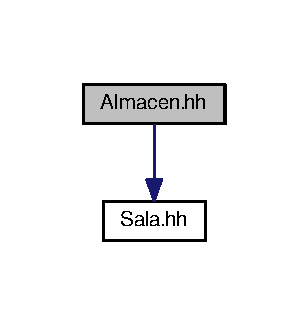
\includegraphics[width=148pt]{_almacen_8hh__incl}
\end{center}
\end{figure}
\subsection*{Clases}
\begin{DoxyCompactItemize}
\item 
class \hyperlink{class_almacen}{Almacen}
\begin{DoxyCompactList}\small\item\em Representa el almacén virtual que contiene en su interior el conjunto completo de salas. A su vez el almacén cuenta con un registro de todos los productos que contiene con sus respectivas cantidades. \end{DoxyCompactList}\end{DoxyCompactItemize}


\subsection{Descripción detallada}
Especificación de la clase \hyperlink{class_almacen}{Almacen}. 


\hypertarget{pro2_8cc}{}\section{Referencia del Archivo pro2.\+cc}
\label{pro2_8cc}\index{pro2.\+cc@{pro2.\+cc}}


Programa principal.  


Dependencia gráfica adjunta para pro2.\+cc\+:\nopagebreak
\begin{figure}[H]
\begin{center}
\leavevmode
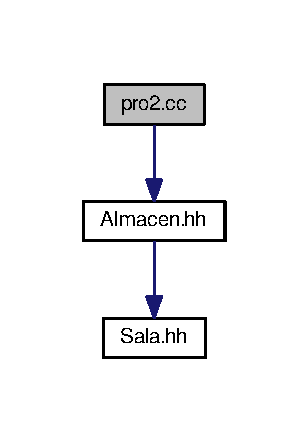
\includegraphics[width=148pt]{pro2_8cc__incl}
\end{center}
\end{figure}
\subsection*{Funciones}
\begin{DoxyCompactItemize}
\item 
int \hyperlink{pro2_8cc_ae66f6b31b5ad750f1fe042a706a4e3d4}{main} ()
\end{DoxyCompactItemize}


\subsection{Descripción detallada}
Programa principal. 

El programa incluye, para una serie de datos incorrectos específicos, un detector de error. Esto implica que si el usuario intenta realizar ciertas operaciones que no cumplan unas determinadas condiciones (como por ejemplo introducir productos no registrados) el programa informará de la existencia de un error.

Pese a lo previamente citado, suponemos que el usuario introduce datos correctos relativos al acceso a salas ya que no hay control respecto a si accedemos a salas inexistentes o se introducen cantidades negativas. 

\subsection{Documentación de las funciones}
\index{pro2.\+cc@{pro2.\+cc}!main@{main}}
\index{main@{main}!pro2.\+cc@{pro2.\+cc}}
\subsubsection[{\texorpdfstring{main()}{main()}}]{\setlength{\rightskip}{0pt plus 5cm}int main (
\begin{DoxyParamCaption}
{}
\end{DoxyParamCaption}
)}\hypertarget{pro2_8cc_ae66f6b31b5ad750f1fe042a706a4e3d4}{}\label{pro2_8cc_ae66f6b31b5ad750f1fe042a706a4e3d4}


Definición en la línea 31 del archivo pro2.\+cc.


\begin{DoxyCode}
31            \{
32 
33   \textcolor{keywordtype}{int} N;                \textcolor{comment}{// Cantidad de salas.}
34   cin >> N;
35   
36   \hyperlink{class_almacen}{Almacen} A(N);            \textcolor{comment}{// Creación y lectura en preorden de la estructura del almacén (con
       identificadores de sala).}
37   
38   A.lectura\_dimensiones\_salas();    \textcolor{comment}{// Lectura de las dimensiones de cada una de las salas.}
39   
40   \textcolor{keywordtype}{string} op;              \textcolor{comment}{// Código de operación.}
41   
42   \textcolor{keywordflow}{while} (cin >> op and op != \textcolor{stringliteral}{"fin"}) \{
43     
44     cout << op;
45     
46     \textcolor{keywordflow}{if} (op == \textcolor{stringliteral}{"poner\_prod"}) \{
47       \textcolor{keywordtype}{string} prod;
48       cin >> prod;
49       
50       cout <<\textcolor{charliteral}{' '} << prod << endl;
51       A.poner\_prod(prod);
52     \}
53     \textcolor{keywordflow}{else} \textcolor{keywordflow}{if} (op == \textcolor{stringliteral}{"quitar\_prod"}) \{
54       \textcolor{keywordtype}{string} prod;
55       cin >> prod;
56       
57       cout <<\textcolor{charliteral}{' '} << prod << endl;
58       A.quitar\_prod(prod);
59     \}
60     \textcolor{keywordflow}{else} \textcolor{keywordflow}{if} (op == \textcolor{stringliteral}{"poner\_items"}) \{
61       \textcolor{keywordtype}{int} sala, cant;
62       \textcolor{keywordtype}{string} prod;
63       cin >> sala >> prod >> cant;
64       
65       cout <<\textcolor{charliteral}{' '} << sala << prod << cant << endl;
66       
67       \textcolor{keywordtype}{int} result = A.poner\_items(sala, prod, cant);
68       \textcolor{keywordflow}{if} (result == -1) cout << \textcolor{stringliteral}{"  error"} << endl;
69       \textcolor{keywordflow}{else} cout <<\textcolor{stringliteral}{"  "} << result << endl;
70     \}
71     \textcolor{keywordflow}{else} \textcolor{keywordflow}{if} (op == \textcolor{stringliteral}{"quitar\_items"}) \{
72       \textcolor{keywordtype}{int} sala, cant;
73       \textcolor{keywordtype}{string} prod;
74       cin >> sala >> prod >> cant;
75       
76       cout <<\textcolor{charliteral}{' '} << sala << prod << cant << endl;
77       
78       \textcolor{keywordtype}{int} result = A.quitar\_items(sala, prod, cant);
79       \textcolor{keywordflow}{if} (result == -1) cout << \textcolor{stringliteral}{"  error"} << endl;
80       \textcolor{keywordflow}{else} cout <<\textcolor{stringliteral}{"  "} << result << endl;
81       
82     \}
83     \textcolor{keywordflow}{else} \textcolor{keywordflow}{if} (op == \textcolor{stringliteral}{"distribuir"}) \{
84       \textcolor{keywordtype}{int} cant;
85       \textcolor{keywordtype}{string} prod;
86       cin >> prod >> cant;
87       
88       cout <<\textcolor{charliteral}{' '} << prod << cant << endl;
89       
90       \textcolor{keywordtype}{int} result = A.distribuir(prod, cant);
91       \textcolor{keywordflow}{if} (result == -1) cout << \textcolor{stringliteral}{"  error"} << endl;
92       \textcolor{keywordflow}{else} cout <<\textcolor{stringliteral}{"  "} << result << endl;
93       
94     \}
95     \textcolor{keywordflow}{else} \textcolor{keywordflow}{if} (op == \textcolor{stringliteral}{"compactar"}) \{
96       \textcolor{keywordtype}{int} sala;
97       cin >> sala;
98       
99       cout <<\textcolor{charliteral}{' '} << sala << endl;
100       A.compactar(sala);
101     \}
102     \textcolor{keywordflow}{else} \textcolor{keywordflow}{if} (op == \textcolor{stringliteral}{"reorganizar"}) \{
103       \textcolor{keywordtype}{int} sala;
104       cin >> sala;
105       
106       cout <<\textcolor{charliteral}{' '} << sala << endl;
107       A.reorganizar(sala);
108     \}
109     \textcolor{keywordflow}{else} \textcolor{keywordflow}{if} (op == \textcolor{stringliteral}{"redimensionar"}) \{
110       \textcolor{keywordtype}{int} sala, fil, col;
111       cin >> sala >> fil >>col;
112       
113       cout <<\textcolor{charliteral}{' '} << sala << fil << col << endl;
114       \textcolor{keywordflow}{if} (not A.redimensionar(sala, fil, col)) cout << \textcolor{stringliteral}{"  error"} << endl;
115     \}
116     \textcolor{keywordflow}{else} \textcolor{keywordflow}{if} (op == \textcolor{stringliteral}{"inventario"}) \{
117       
118       A.inventario();
119     \}
120     \textcolor{keywordflow}{else} \textcolor{keywordflow}{if} (op == \textcolor{stringliteral}{"escribir"}) \{
121       \textcolor{keywordtype}{int} sala;
122       cin >> sala;
123       
124       cout <<\textcolor{charliteral}{' '} << sala << endl;
125       A.escribir(sala);
126     \}
127     \textcolor{keywordflow}{else} \textcolor{keywordflow}{if} (op == \textcolor{stringliteral}{"consultar\_pos"}) \{
128       \textcolor{keywordtype}{int} sala, fil, col;
129       cin >> sala >> fil >>col;
130       
131       cout <<\textcolor{charliteral}{' '} << sala << fil << col << endl;
132       cout <<\textcolor{stringliteral}{"  "} << A.consultar\_pos(sala, fil, col) << endl;
133     \}
134     \textcolor{keywordflow}{else} \textcolor{keywordflow}{if} (op == \textcolor{stringliteral}{"consultar\_prod"}) \{
135       \textcolor{keywordtype}{string} prod;
136       cin >> prod;
137       
138       cout <<\textcolor{charliteral}{' '} << prod << endl;
139       \textcolor{keywordtype}{int} result = A.consultar\_prod(prod);
140       
141       \textcolor{keywordflow}{if} (result == -1) cout << \textcolor{stringliteral}{"  error"} << endl;
142       \textcolor{keywordflow}{else} cout <<\textcolor{stringliteral}{"  "} << result << endl;
143     \}
144   \}
145   
146   cout << op << endl;
147 \}
\end{DoxyCode}

\hypertarget{_sala_8hh}{}\section{Referencia del Archivo Sala.\+hh}
\label{_sala_8hh}\index{Sala.\+hh@{Sala.\+hh}}


Especificación de la clase \hyperlink{class_sala}{Sala}.  


\subsection*{Clases}
\begin{DoxyCompactItemize}
\item 
class \hyperlink{class_sala}{Sala}
\begin{DoxyCompactList}\small\item\em Representa una sala virtual asociada a un identificador y que contiene una estantería junto a datos relacionadas con la misma\+: dimensiones, espacio ocupado y espacio máximo. \end{DoxyCompactList}\end{DoxyCompactItemize}


\subsection{Descripción detallada}
Especificación de la clase \hyperlink{class_sala}{Sala}. 


%--- End generated contents ---

% Index
\backmatter
\newpage
\phantomsection
\clearemptydoublepage
\addcontentsline{toc}{chapter}{Índice}
\printindex

\end{document}
